\appendix
\chapter{Arquitectura del Sistema}

En este apartado se presenta la representación visual de la arquitectura del sistema, detallando el flujo de comunicación entre los diversos componentes tecnológicos que conforman la solución.

\begin{figure}[htbp]
    \centering
    % Aquí debes reemplazar 'ruta/a/tu/imagen' por el nombre real de tu archivo de imagen
    % (ej. arquitectura_sircar.png)
    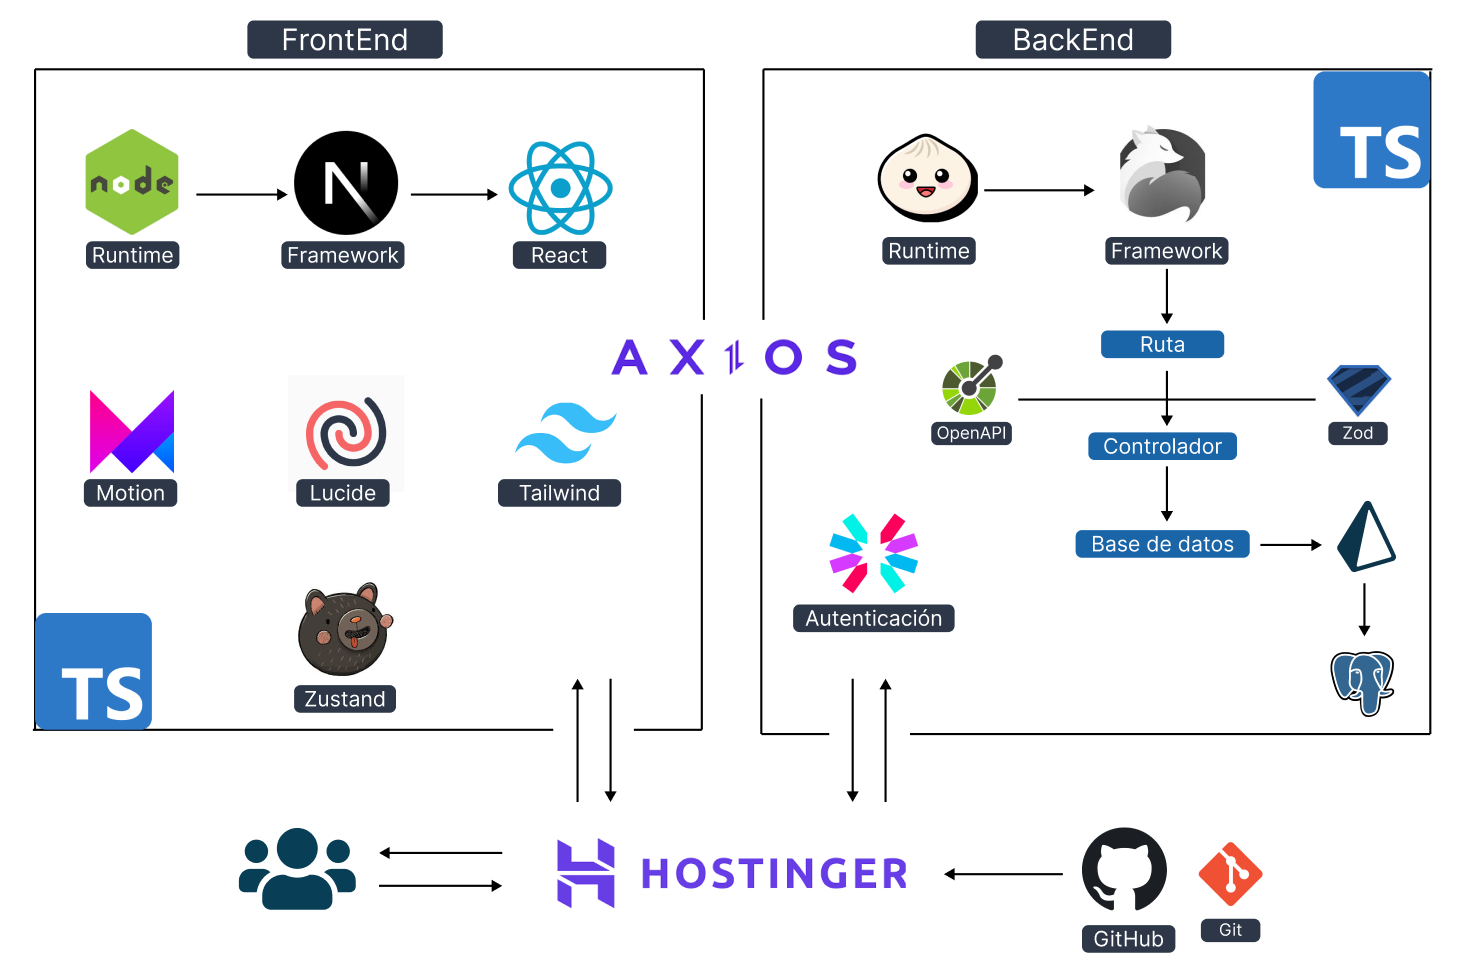
\includegraphics[width=0.9\textwidth]{imagenes/arquitectura.png}
    \caption{Diagrama de arquitectura del sistema: Flujo de comunicación y componentes tecnológicos.}
    \label{fig:arquitectura_general}
\end{figure}

\section{Descripción de los componentes}
La arquitectura se fundamenta en un esquema del frontends y backend, diseñado para garantizar escalabilidad y modularidad:

\begin{itemize}
    \item \textbf{Frontend:} Desarrollado con Next.js y Tailwind CSS, optimizado para una navegación fluida entre las distintas secciones de gestión.
    \item \textbf{Backend:} Implementado con el runtime Bun y el framework Elysia, proporcionando una API de alto rendimiento.
    \item \textbf{Persistencia de datos:} PostgreSQL gestionado como base de datos central, asegurando la integridad de la información clínica y de usuarios.
    \item \textbf{Infraestructura:} Despliegue gestionado mediante la plataforma Dokploy, permitiendo la contenerización y orquestación eficiente de los servicios en un entorno de servidor VPS.
\end{itemize}

El diagrama ilustra mediante flechas el flujo de datos: las peticiones del cliente son procesadas por la API, la cual interactúa directamente con la base de datos para la persistencia, manteniendo una separación clara de responsabilidades que facilita el mantenimiento y la escalabilidad del sistema.